\documentclass{article}
\usepackage[utf8]{inputenc}
\usepackage[margin=1.0in]{geometry}
\usepackage{graphicx}
\usepackage{wrapfig}
\usepackage{amsmath}
\usepackage{subfig}
\usepackage[makeroom]{cancel}
\let\vec\mathbf
\usepackage{float}

\title{Stereo Imaging}
\author{Saketh Gabbita, Adapted from George Tang}
\date{November 20, 2019}

\begin{document}

\maketitle

\section{Introduction}
Many applications in computational photography requires knowing the depth of objects in an image. For instance, the scattering of light by fog can be modeled as a function of depth. Computing the "depth map" of an image taken in fog and using it in conjunction with atmospheric scattering physics allows us to "defog" the image. 

The depth map is a matrix, where every entry represents the distance (e.g. meters) of the source emitting the color captured by the pixel. The depth map can be visualized by scaling every value within the 0-255 range, so it becomes a grayscale image. 

\section{Depth from Disparity}
To approach this problem, we look towards the human vision system for inspiration. Humans have two eyes, each with presenting the brain a slightly offset worldview (put your finger in front of you and close one eye at a time; you'll notice the finger shifts). The brain uses this offset the perceive depth. 

We can replicate this phenomena using two cameras. This setup is known as a \textit{stereo camera system}. We assume an \textit{equipolar constraint}, or the cameras are placed on level surfaces. Notice below in Figure 1 b, the image taken by the left lens to shifted towards the right compared to the image taken by the right lens. Most of the pixels in the right image has a corresponding pixel to the right in the left image. If we compute this difference (a.k.a disparity), we get the disparity map. 

\begin{figure}[!htbp]
 \centering
    \subfloat[Stereo Camera]{{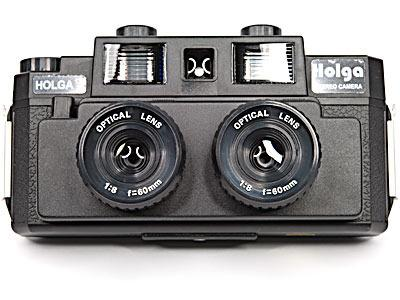
\includegraphics[width=5.5cm]{stereocam.jpg} }}%
    \qquad
    \subfloat[Disparity Map from Two Images]{{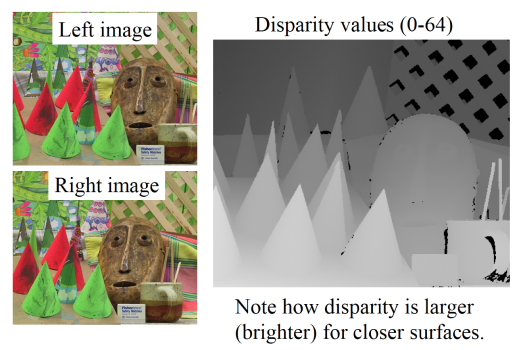
\includegraphics[width=5.5cm]{img1.png} }}%
    \caption{The workings of stereo vision}%
    \label{fig:example}%
\end{figure}

The disparity is inversely related to the depth map. Larger disparity means the object is closer (again try experimenting with your finger and eyes). This means in areas where the disparity is the brightest, the depth map is the darkest (this can be inverted with color transformations). 

We can derive this inverse relation using similar triangles. Observe the figure on the text page, which places the image planes of each camera parallel to the x-y plane, with the bottom left of the left camera at the origin. We can obtain the x-y coordinates of the projection of the object for each image. Again, if the cameras are level, the y coordinates are the same, and the disparity will simply be the difference in x coordinates. 

\begin{minipage}{.35\textwidth}
Notice that $Z$ in the diagram to the right is the depth. $f$ we define to be the distance the image planes are from the x-y plane (a.k.a focal length of the camera). $T_x$ is the distance between the lower left corners of the image planes, which is equivalent to the distance between the lenses.

    $$ d = x_l-x_r$$
    
    $$ d = f\frac{X}{Z} - f\frac{X-T_x}{Z}$$
    
    $$ d = \frac{fT_x}{Z}$$


\end{minipage}
\hspace{20pt}
\begin{minipage}{.65\textwidth}
\begin{center}
    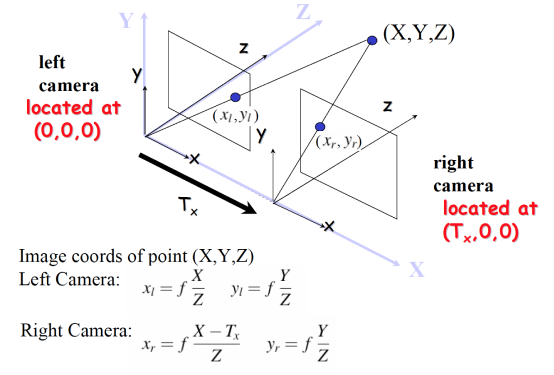
\includegraphics[width=1\textwidth]{cam1.png}
  \end{center}
\end{minipage}

\section{Naive Matching}
We now have established that we can obtain the depth map from the disparity map. Notice that pixels in a row in the right image only correspond to pixels in the same row in the left image. Thus, if we define a dissimilarity function of two patches, each centered around the corresponding pixels in a proposed pair, or a cost function of matching two patches, we can find the minimum cost, and that proposed pair will be the actual corresponding pixels. 

The cost function, $M(l, r)$, is usually the $SSD$ (sum of sqaured differences) or $0.5(1-NCC)$ for better performance where NCC is the normalized cross-correlation (value between -1 and 1). 

\begin{center}
    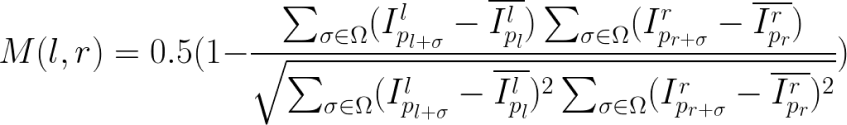
\includegraphics[width=0.5\textwidth]{NCC.png}
\end{center}

where $\overline{I}$ represents the mean, superscripts the image (left, right), and $p_l$, $P_r$ the respective patch.

Naive matching produces very poor results. Two issues are that the mapping is not one-to-one, meaning that one pixel can match to many corresponding pixels, and there are many false occlusions (areas visible in only one image). Below are some examples using different size patches (black areas represent occlusions).

\begin{center}
    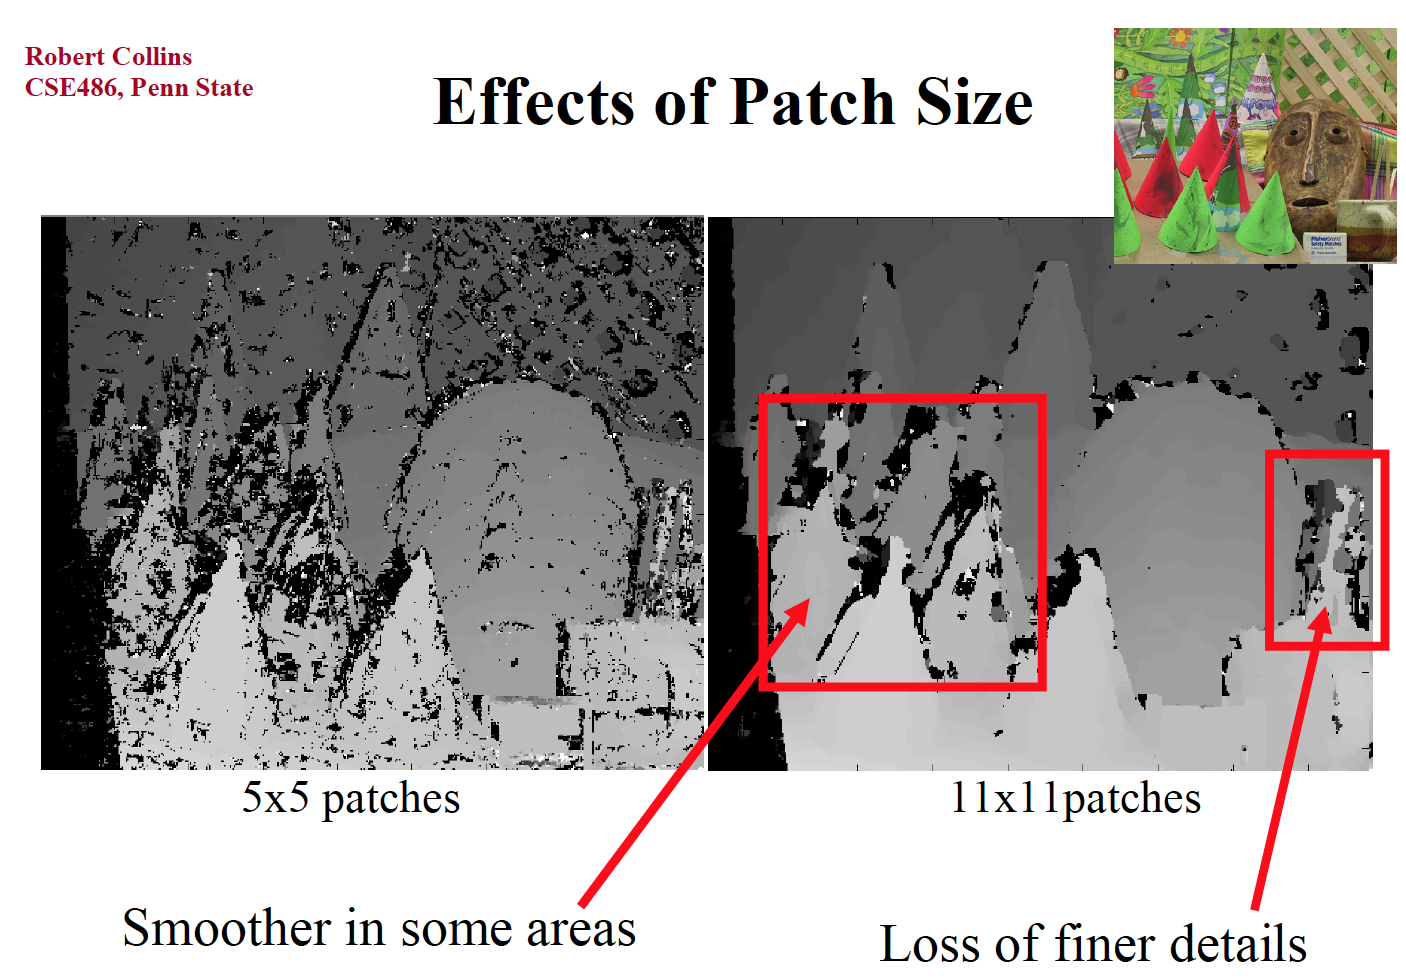
\includegraphics[width=0.65\textwidth]{patch.png}
\end{center}

\section{3 State Dynamic Programming}
Before we discuss better methods, we introduce the DSI (Disparity Space Image). When we perform naive matching, we computed for every pixel the cost of matching with every pixel in the corresponding row in the other image. If we insert every possible matching combination of a row into a matrix, we get the DSI, where DSI[i, j] is the cost of matching the ith pixel against the jth pixel of the corresponding row. 

\begin{figure}[!htbp]
 \centering
    \subfloat[Computing the DSI]{{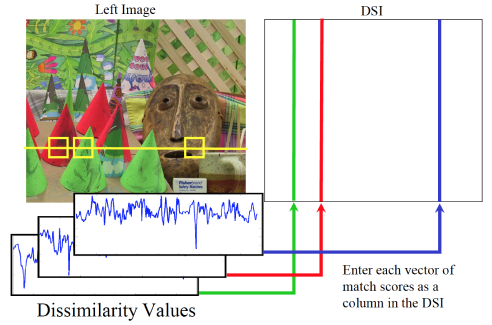
\includegraphics[width=7cm]{IMGDSI.png} }}%
    \qquad
    \subfloat[Examples of the min cost path]{{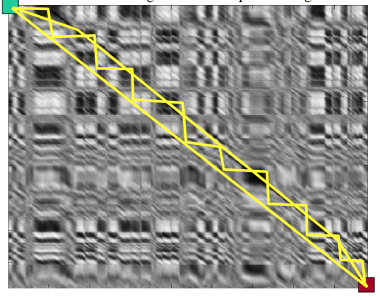
\includegraphics[width=5.5cm]{DSI.png} }}%
    \label{fig:example}%
\end{figure}

In 1998, Cox et al proposed a global method for computing each row of the disparity map separately using a global method. Given a DSI for each row, we want to minimize the overall cost of matching where each pixel is matched to at most one pixel or otherwise defined as an occlusion (no matching). We can accomplish this using dynamic programming with 3 states and 3 transitions. 

\begin{center}
    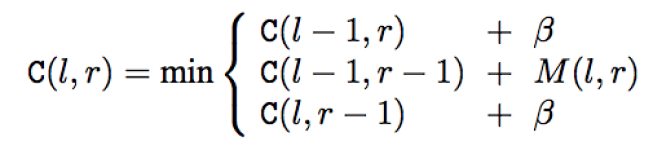
\includegraphics[width=0.4\textwidth]{DP3.png}
\end{center}

\begin{center}
    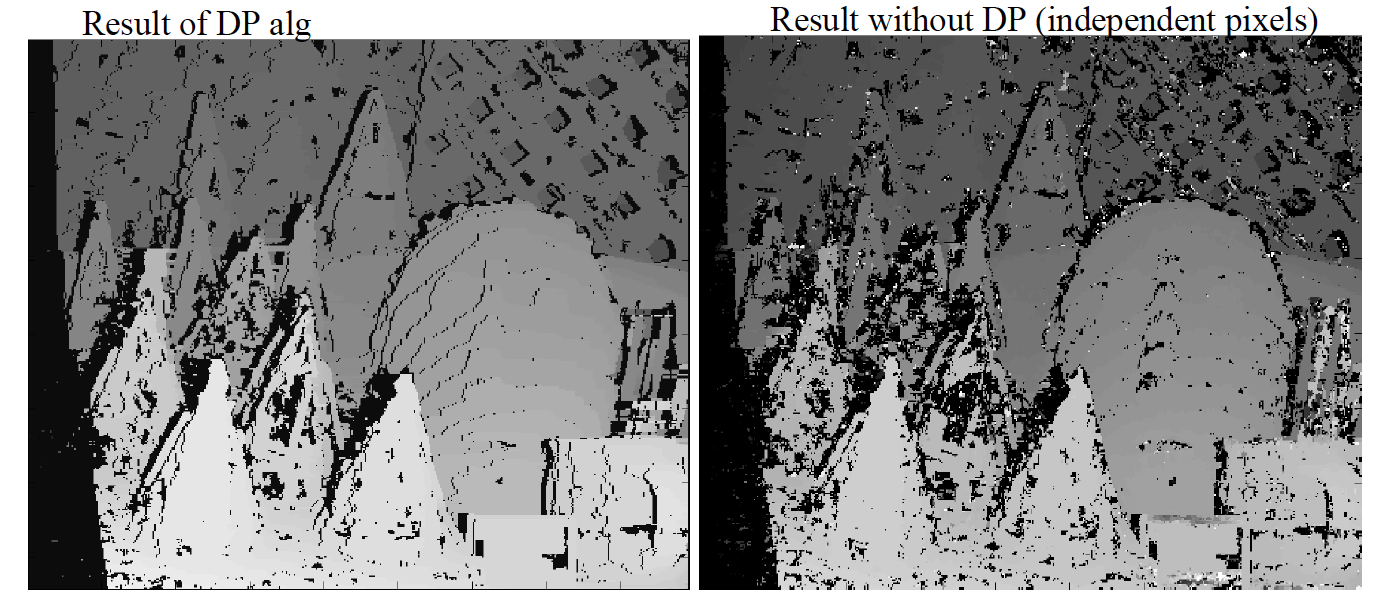
\includegraphics[width=0.7\textwidth]{DPdemo.png}
\end{center}

As you can see, performance doesn't improve as much.

\section{4 State Dynamic Programming}
In 2006, researchers at Microsoft proposed a 4 state DP model with 14 transitions that greatly improves the quality of the disparity maps. On the next page is the formulation for the DP. The transitions for $R_o$ and $R_m$ can be determined through symmetry.

\begin{center}
    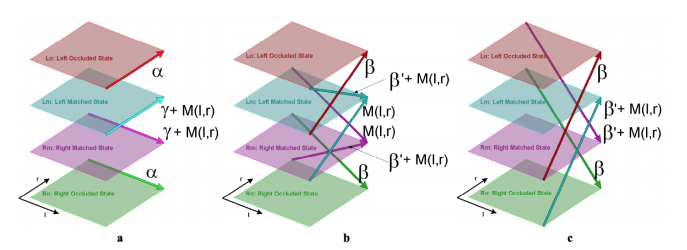
\includegraphics[width=0.9\textwidth]{DP4I.png}
\end{center}

\begin{center}
    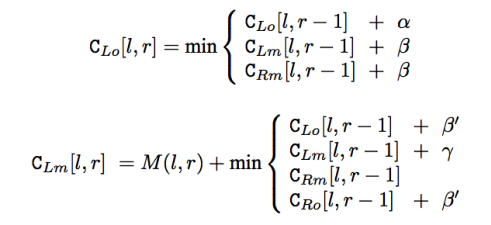
\includegraphics[width=0.5\textwidth]{DP4.png}
\end{center}

\section{Parallelization and Improvements}
Because each row is processed independently of other rows, we the problem of computing the disparity map is embarrassingly parallel. However, this also leaks to streaks across the disparity maps because information is not propagated between rows. To fix this, researchers who proposed the 4 State DP also proposed precomputing the DIS, stacking them in a 3D structure as shown below, and then applying a Gaussian blur across the diagonal before computing the min cost path. Doing so rids of many streaks (see 3 images below).

\begin{center}
    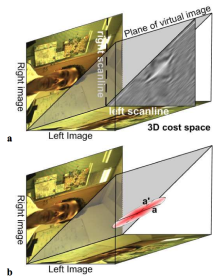
\includegraphics[width=0.2\textwidth]{blur.png}
\end{center}

\begin{figure}[!htbp]
 \centering
    \subfloat[3 State DP]{{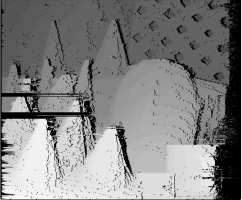
\includegraphics[width=4cm]{3.png} }}%
    \qquad
    \subfloat[3 State DP with Blur]{{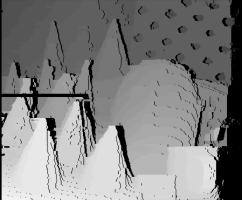
\includegraphics[width=4cm]{3B.png} }}%
    \label{fig:example}%
    \qquad
    \subfloat[4 State DP with Blur]{{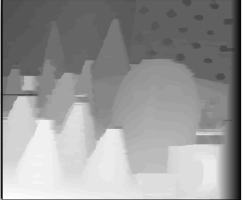
\includegraphics[width=4cm]{4.png} }}%
    \label{fig:example}%
\end{figure}

\end{document}
